\documentclass[12pt,a4paper]{article}

% ─── Packages ───────────────────────────────────────────────────────────────
\usepackage{amsmath}
\usepackage{amssymb}
\usepackage{geometry}
\geometry{margin=2.5cm}
\usepackage{booktabs}
\usepackage{xcolor}
\usepackage{hyperref}
\usepackage{listings}
\usepackage{pgfplots}
\pgfplotsset{compat=1.18}
\usepackage{tcolorbox}
\tcbuselibrary{skins, breakable}
\usepackage{enumitem}
\usepackage{fancyhdr}
\usepackage{tikz}
\usepackage{array}

% ─── tcolorbox environments ──────────────────────────────────────────────────
\newtcolorbox{curiositybox}[1]{colback=yellow!10, colframe=orange!80!black, fonttitle=\bfseries, title=#1, breakable}
\newtcolorbox{infobox}[1]{colback=blue!5, colframe=blue!60!black, fonttitle=\bfseries, title=#1, breakable}
\newtcolorbox{mistakebox}[1]{colback=red!5, colframe=red!60!black, fonttitle=\bfseries, title=#1, breakable}
\newtcolorbox{learnbox}[1]{colback=green!5, colframe=green!60!black, fonttitle=\bfseries, title=#1, breakable}

% ─── lstlisting (Python) ─────────────────────────────────────────────────────
\lstset{language=Python, basicstyle=\ttfamily\small, keywordstyle=\color{blue},
        commentstyle=\color{gray}, stringstyle=\color{orange},
        showstringspaces=false, numbers=left, numberstyle=\tiny,
        breaklines=true, frame=single}

% ─── fancyhdr ────────────────────────────────────────────────────────────────
\pagestyle{fancy}
\fancyhf{}
\lhead{Topic 05: Derivatives \& Integrals}
\rhead{Unit IV --- Laplace Transforms}
\cfoot{\thepage}

% ─── Title ───────────────────────────────────────────────────────────────────
\title{Topic 05: Transforms of Derivatives and Integrals \\
       \large Unit IV --- Laplace Transforms}
\author{JNTUA College of Engineering (Autonomous)\\
        23A54201 --- Mathematics IV (Transform Techniques)}
\date{}

% ─────────────────────────────────────────────────────────────────────────────
\begin{document}
\maketitle
\tableofcontents
\newpage

% =============================================================================
\section{Opening Hook}
% =============================================================================

\begin{curiositybox}{Hook}
Here is the single sentence that makes the entire Laplace method worth learning:
differentiation in the time domain becomes MULTIPLICATION by \(s\) in the transform domain.
A second-order differential equation --- the kind that normally takes pages of integration
and constant-solving --- turns into a one-line algebra problem.
This is the topic where calculus finally surrenders to algebra.
\end{curiositybox}

% =============================================================================
\section{Why This Topic Exists}
% =============================================================================

Before we begin, here is the honest answer to why you are reading this.
Every other topic in Unit IV --- standard forms, existence conditions, inverse transforms,
shifting theorems --- is really preparation for \emph{this} topic.
The Laplace transform was invented precisely to convert differential equations (hard)
into algebraic equations (easy).
Without the derivative and integral transform rules, the entire framework is a beautiful
mathematical curiosity with no practical payoff.

\medskip
\noindent The table below shows three common mistakes and their consequences when you
ignore or mis-apply the formulas in this topic.

\begin{center}
\begin{tabular}{p{6cm} p{7cm}}
\toprule
\textbf{Mistake} & \textbf{Consequence} \\
\midrule
Forgetting initial condition terms in the derivative formula
  & Getting the wrong particular solution entirely \\[4pt]
Confusing \(f'(0)\) with \(F'(s)\)
  & Mixing up time-domain and \(s\)-domain quantities \\[4pt]
Skipping the integral transform rule
  & Being unable to solve integro-differential equations \\
\bottomrule
\end{tabular}
\end{center}

\begin{learnbox}{Why This Topic Is Central}
This topic is the bridge between the abstract definition of the Laplace transform and its
real engineering utility.
Master these two rules --- derivative transform and integral transform --- and you can solve
virtually every ODE that appears in your syllabus.
\end{learnbox}

% =============================================================================
\section{You Already Know This (Intuition First)}
% =============================================================================

Think of the Laplace transform as a translator between two languages.
In everyday speech, you might say: ``the rate of change of my bank balance is \$200 per month.''
That is a calculus statement --- an ongoing process in time.
A translator fluent in \emph{algebra} would instead write a single symbol: multiply the
balance-transform by \(s\).
The messy, continuous, time-based verb (``rate of change'') becomes a compact algebraic noun.

Calculus operations are \emph{verbs}: they describe something happening over time ---
a function growing, oscillating, accumulating.
The Laplace transform turns those verbs into simple algebraic \emph{nouns} in the \(s\)-domain:
\begin{itemize}
  \item Differentiation (the verb ``take the derivative'') $\longrightarrow$ multiply by \(s\) (and subtract initial values).
  \item Integration (the verb ``accumulate area'') $\longrightarrow$ divide by \(s\).
\end{itemize}
Once you see this, the method feels almost obvious in hindsight.

% =============================================================================
\section{Transform of the First Derivative}
% =============================================================================

\begin{infobox}{Theorem: \(\mathcal{L}\{f'(t)\} = sF(s) - f(0)\)}
\textbf{Statement:} If \(f(t)\) is continuous, of exponential order, and \(f'(t)\) is piecewise
continuous on \([0,\infty)\), then
\[
  \mathcal{L}\{f'(t)\} = sF(s) - f(0).
\]

\textbf{Derivation from the definition:}
\[
  \mathcal{L}\{f'(t)\} = \int_0^\infty e^{-st}\,f'(t)\,dt.
\]
Apply integration by parts with \(u = e^{-st}\) and \(dv = f'(t)\,dt\):
\[
  du = -s\,e^{-st}\,dt, \qquad v = f(t).
\]
Therefore
\[
  \int_0^\infty e^{-st}\,f'(t)\,dt
  = \Bigl[e^{-st}\,f(t)\Bigr]_0^\infty
    - \int_0^\infty (-s)\,e^{-st}\,f(t)\,dt.
\]
Evaluate the boundary term:
\begin{itemize}
  \item As \(t \to \infty\): because \(f(t)\) is of exponential order \(\alpha\) and
        \(\operatorname{Re}(s) > \alpha\), the term \(e^{-st}\,f(t) \to 0\).
  \item At \(t = 0\): \(e^{-s \cdot 0}\,f(0) = f(0)\).
\end{itemize}
Hence the boundary term equals \(0 - f(0) = -f(0)\).
The remaining integral is
\[
  s\int_0^\infty e^{-st}\,f(t)\,dt = s\,F(s).
\]
Combining:
\[
  \boxed{\mathcal{L}\{f'(t)\} = sF(s) - f(0).}
\]
\end{infobox}

\begin{learnbox}{What Did We Learn?}
The first-derivative transform rule converts differentiation into multiplication by \(s\),
but carries a ``memory'' of the initial value \(f(0)\).
If \(f(0)=0\) the rule simplifies to \(\mathcal{L}\{f'(t)\}=sF(s)\).
\end{learnbox}

% =============================================================================
\section{Transform of the Second Derivative}
% =============================================================================

\begin{infobox}{Theorem: \(\mathcal{L}\{f''(t)\} = s^2F(s) - sf(0) - f'(0)\)}
\textbf{Derivation by applying the first-derivative rule twice:}

Let \(g(t) = f'(t)\).
Then \(g'(t) = f''(t)\), \(g(0) = f'(0)\), and
\(\mathcal{L}\{g(t)\} = \mathcal{L}\{f'(t)\} = sF(s) - f(0)\).

Apply the first-derivative formula to \(g\):
\[
  \mathcal{L}\{f''(t)\}
  = \mathcal{L}\{g'(t)\}
  = s\,\mathcal{L}\{g(t)\} - g(0)
  = s\,\bigl[sF(s) - f(0)\bigr] - f'(0).
\]
Expand:
\[
  = s^2F(s) - s\,f(0) - f'(0).
\]
\[
  \boxed{\mathcal{L}\{f''(t)\} = s^2F(s) - sf(0) - f'(0).}
\]
Notice that the formula ``remembers'' both initial conditions: the value \(f(0)\) and the
initial slope \(f'(0)\).
These are precisely the two constants you would need to specify when solving a second-order
ODE using classical methods.
\end{infobox}

\begin{learnbox}{What Did We Learn?}
The second-derivative rule requires \emph{both} \(f(0)\) and \(f'(0)\).
These are the initial conditions from the original ODE problem statement ---
they are not computed from \(F(s)\); they are \emph{given data}.
\end{learnbox}

% =============================================================================
\section{General \texorpdfstring{$n$}{n}th Derivative Formula}
% =============================================================================

\begin{infobox}{General nth Derivative Rule}
By repeatedly applying the first-derivative formula, one obtains:
\[
  \mathcal{L}\{f^{(n)}(t)\}
  = s^n F(s) - s^{n-1}f(0) - s^{n-2}f'(0) - \cdots - f^{(n-1)}(0).
\]
The pattern is:
\begin{itemize}
  \item Lead term: \(s^n F(s)\).
  \item Then subtract \(s^{n-1}f(0), s^{n-2}f'(0), \ldots, s^0 f^{(n-1)}(0)\) --- powers of \(s\) decrease from \(n-1\) down to \(0\), paired with successive initial conditions.
\end{itemize}

\medskip
The explicit formulas for \(n = 1\) through \(5\) are:

\begin{center}
\begin{tabular}{c l}
\toprule
\(n\) & \(\mathcal{L}\{f^{(n)}(t)\}\) \\
\midrule
1 & \(sF(s) - f(0)\) \\
2 & \(s^2F(s) - sf(0) - f'(0)\) \\
3 & \(s^3F(s) - s^2f(0) - sf'(0) - f''(0)\) \\
4 & \(s^4F(s) - s^3f(0) - s^2f'(0) - sf''(0) - f'''(0)\) \\
5 & \(s^5F(s) - s^4f(0) - s^3f'(0) - s^2f''(0) - sf'''(0) - f^{(4)}(0)\) \\
\bottomrule
\end{tabular}
\end{center}
\end{infobox}

\begin{learnbox}{What Did We Learn?}
The general formula is easy to remember: start with \(s^n F(s)\) and subtract
a descending staircase of \(s\)-powers multiplied by successive initial conditions.
Each new derivative order adds exactly one more initial condition term.
\end{learnbox}

% =============================================================================
\section{Transform of an Integral}
% =============================================================================

\begin{infobox}{Theorem: \(\mathcal{L}\left\{\int_0^t f(u)\,du\right\} = \dfrac{F(s)}{s}\)}
\textbf{Derivation using the derivative rule in reverse:}

Define \(g(t) = \int_0^t f(u)\,du\).
Then:
\begin{itemize}
  \item \(g'(t) = f(t)\) \quad (Fundamental Theorem of Calculus).
  \item \(g(0) = \int_0^0 f(u)\,du = 0\).
\end{itemize}
Apply the first-derivative transform rule to \(g(t)\):
\[
  \mathcal{L}\{g'(t)\} = s\,\mathcal{L}\{g(t)\} - g(0)
  \implies
  \mathcal{L}\{f(t)\} = s\,\mathcal{L}\{g(t)\} - 0.
\]
Therefore:
\[
  F(s) = s\,\mathcal{L}\{g(t)\}
  \implies
  \mathcal{L}\{g(t)\} = \frac{F(s)}{s}.
\]
Written explicitly:
\[
  \boxed{\mathcal{L}\!\left\{\int_0^t f(u)\,du\right\} = \frac{F(s)}{s}.}
\]
\end{infobox}

\begin{learnbox}{What Did We Learn?}
Integration in the time domain divides by \(s\) in the \(s\)-domain.
This is the perfect dual of the derivative rule (which multiplies by \(s\)).
Together they confirm that the Laplace transform converts all calculus operations into
elementary algebra.
\end{learnbox}

% =============================================================================
\section{The Real Payoff: Solving ODEs with Initial Conditions}
% =============================================================================

The four-step Laplace ODE method is illustrated in the flowchart below.

\begin{center}
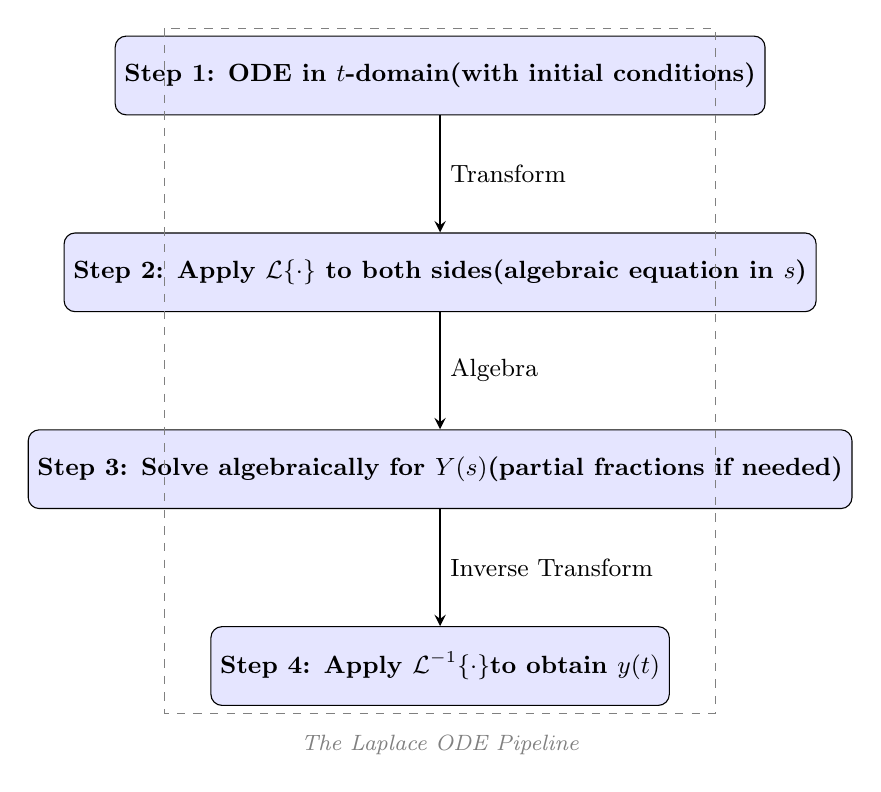
\begin{tikzpicture}[
    box/.style={draw, rounded corners, fill=blue!10,
                minimum width=5cm, minimum height=1cm,
                text centered, font=\small\bfseries},
    arrow/.style={->, thick, >=stealth}
  ]
  % Boxes
  \node[box] (A) at (0,0)   {Step 1: ODE in \(t\)-domain\\(with initial conditions)};
  \node[box] (B) at (0,-2.5){Step 2: Apply \(\mathcal{L}\{\cdot\}\) to both sides\\
                              (algebraic equation in \(s\))};
  \node[box] (C) at (0,-5)  {Step 3: Solve algebraically for \(Y(s)\)\\
                              (partial fractions if needed)};
  \node[box] (D) at (0,-7.5){Step 4: Apply \(\mathcal{L}^{-1}\{\cdot\}\)\\
                              to obtain \(y(t)\)};
  % Arrows
  \draw[arrow] (A) -- node[right, font=\small]{Transform} (B);
  \draw[arrow] (B) -- node[right, font=\small]{Algebra} (C);
  \draw[arrow] (C) -- node[right, font=\small]{Inverse Transform} (D);
  % Side label
  \draw[dashed, gray] (-3.5,0.6) rectangle (3.5,-8.1);
  \node[font=\footnotesize\itshape, gray] at (0,-8.5)
        {The Laplace ODE Pipeline};
\end{tikzpicture}
\end{center}

\begin{infobox}{The 4-Step Laplace Method for ODEs}
\begin{enumerate}
  \item \textbf{Write the ODE} with all initial conditions specified.
  \item \textbf{Take the Laplace transform} of every term.
        Use \(\mathcal{L}\{y'(t)\}=sY(s)-y(0)\) and
        \(\mathcal{L}\{y''(t)\}=s^2Y(s)-sy(0)-y'(0)\).
        The result is an algebraic equation in \(Y(s)\).
  \item \textbf{Solve algebraically for \(Y(s)\)}.
        Group all \(Y(s)\) terms on one side; factor out \(Y(s)\).
        Use partial fraction decomposition as needed.
  \item \textbf{Apply the inverse Laplace transform} to each term of \(Y(s)\)
        to recover \(y(t)\).
\end{enumerate}
\end{infobox}

% =============================================================================
\section{Worked Examples}
% =============================================================================

% ── Example 1 ────────────────────────────────────────────────────────────────
\begin{infobox}{Example 1: First-Order ODE --- \(y' + 3y = e^{2t},\; y(0)=1\)}

\textbf{Step 1.} The ODE is \(y' + 3y = e^{2t}\) with \(y(0)=1\).

\textbf{Step 2. Take the Laplace transform of every term.}
\[
  \mathcal{L}\{y'\} + 3\,\mathcal{L}\{y\} = \mathcal{L}\{e^{2t}\}
\]
\[
  \bigl[sY(s) - y(0)\bigr] + 3Y(s) = \frac{1}{s-2}
\]
Substitute \(y(0)=1\):
\[
  sY(s) - 1 + 3Y(s) = \frac{1}{s-2}
\]
\[
  (s+3)Y(s) = \frac{1}{s-2} + 1 = \frac{1 + (s-2)}{s-2} = \frac{s-1}{s-2}.
\]

\textbf{Step 3. Solve for \(Y(s)\).}
\[
  Y(s) = \frac{s-1}{(s-2)(s+3)}.
\]
Partial fractions: write \(\dfrac{s-1}{(s-2)(s+3)} = \dfrac{A}{s-2} + \dfrac{B}{s+3}\).

Multiply through: \(s-1 = A(s+3) + B(s-2)\).

Set \(s=2\): \(1 = 5A \Rightarrow A = \tfrac{1}{5}\).

Set \(s=-3\): \(-4 = -5B \Rightarrow B = \tfrac{4}{5}\).

\[
  Y(s) = \frac{1/5}{s-2} + \frac{4/5}{s+3}.
\]

\textbf{Step 4. Inverse Laplace transform.}
\[
  y(t) = \tfrac{1}{5}\,e^{2t} + \tfrac{4}{5}\,e^{-3t}.
\]
\end{infobox}

\begin{learnbox}{What Did We Learn? --- Example 1}
The first-order ODE \(y'+3y=e^{2t}\), \(y(0)=1\) reduces in one step to algebra.
Partial fractions split \(Y(s)\) into simple recognisable forms whose inverse transforms
are immediate.
The initial condition \(y(0)=1\) was absorbed automatically --- no ``particular + homogeneous''
splitting was needed.
\end{learnbox}

% ── Example 2 ────────────────────────────────────────────────────────────────
\begin{infobox}{Example 2: Second-Order ODE --- \(y'' - 3y' + 2y = 0,\; y(0)=1,\; y'(0)=0\)}

\textbf{Step 1.} The ODE is \(y'' - 3y' + 2y = 0\) with \(y(0)=1\), \(y'(0)=0\).

\textbf{Step 2. Transform every term.}
\[
  \mathcal{L}\{y''\} - 3\,\mathcal{L}\{y'\} + 2\,\mathcal{L}\{y\} = 0
\]
\[
  \bigl[s^2Y(s) - sy(0) - y'(0)\bigr]
  - 3\bigl[sY(s) - y(0)\bigr]
  + 2Y(s) = 0.
\]
Substitute \(y(0)=1\), \(y'(0)=0\):
\[
  s^2Y(s) - s - 0 - 3sY(s) + 3 + 2Y(s) = 0
\]
\[
  (s^2 - 3s + 2)\,Y(s) = s - 3.
\]

\textbf{Step 3. Solve for \(Y(s)\).}
\[
  Y(s) = \frac{s-3}{s^2 - 3s + 2} = \frac{s-3}{(s-1)(s-2)}.
\]
Partial fractions: \(\dfrac{s-3}{(s-1)(s-2)} = \dfrac{A}{s-1} + \dfrac{B}{s-2}\).

Multiply: \(s-3 = A(s-2)+B(s-1)\).

Set \(s=1\): \(-2 = -A \Rightarrow A=2\).

Set \(s=2\): \(-1 = B \Rightarrow B=-1\).

\[
  Y(s) = \frac{2}{s-1} - \frac{1}{s-2}.
\]

\textbf{Step 4. Inverse transform.}
\[
  y(t) = 2e^{t} - e^{2t}.
\]

\textbf{Verification:} \(y(0) = 2-1=1\checkmark\);
\(y'(t)=2e^t-2e^{2t}\), so \(y'(0)=2-2=0\checkmark\).
\end{infobox}

\begin{learnbox}{What Did We Learn? --- Example 2}
For a second-order ODE with zero right-hand side, the Laplace method still works perfectly.
Both initial conditions appear automatically on the left after transforming.
The final answer \(y(t)=2e^t - e^{2t}\) can be verified instantly by back-substitution.
\end{learnbox}

% ── Example 3 ────────────────────────────────────────────────────────────────
\begin{infobox}{Example 3: Integral Equation --- \(y(t) = t + \int_0^t y(u)\sin(t-u)\,du\)}

\textbf{Step 1.} The equation is
\[
  y(t) = t + \int_0^t y(u)\sin(t-u)\,du.
\]
The integral \(\int_0^t y(u)\sin(t-u)\,du\) is a convolution of \(y(t)\) and \(\sin t\).

\textbf{Step 2. Take \(\mathcal{L}\{\cdot\}\) of both sides.}

Using \(\mathcal{L}\{t\} = \dfrac{1}{s^2}\) and the integral (convolution) property
\(\mathcal{L}\{\text{convolution}\} = Y(s)\cdot\mathcal{L}\{\sin t\} = Y(s)\cdot\dfrac{1}{s^2+1}\):
\[
  Y(s) = \frac{1}{s^2} + Y(s)\cdot\frac{1}{s^2+1}.
\]

\textbf{Step 3. Solve for \(Y(s)\).}
\[
  Y(s)\left(1 - \frac{1}{s^2+1}\right) = \frac{1}{s^2}
\]
\[
  Y(s)\cdot\frac{s^2}{s^2+1} = \frac{1}{s^2}
\]
\[
  Y(s) = \frac{s^2+1}{s^4}.
\]
Expand:
\[
  Y(s) = \frac{1}{s^2} + \frac{1}{s^4}.
\]

\textbf{Step 4. Inverse transform.}

Using \(\mathcal{L}^{-1}\!\left\{\dfrac{1}{s^n}\right\} = \dfrac{t^{n-1}}{(n-1)!}\):
\[
  y(t) = t + \frac{t^3}{6}.
\]
\end{infobox}

\begin{learnbox}{What Did We Learn? --- Example 3}
An integral equation (not even an ODE!) yields to the Laplace method immediately.
The convolution inside the integral becomes a simple product in the \(s\)-domain.
After algebra, the inverse transform gives the exact closed-form solution \(y(t)=t+\tfrac{t^3}{6}\).
\end{learnbox}

% =============================================================================
\section{Excel Example}
% =============================================================================

\begin{infobox}{Excel: Verifying Example 2 Numerically (\(y(t)=2e^t - e^{2t}\))}

\textbf{Setup.} From Example 2, the closed-form solution is \(y(t)=2e^t-e^{2t}\).
We verify it against a simple Euler step approximation of \(y''-3y'+2y=0\),
\(y(0)=1\), \(y'(0)=0\).

For Euler's method on a second-order ODE, let \(v=y'\).
The system is \(y' = v\), \(v' = 3v - 2y\).
Step size \(h=0.5\).

\medskip
\noindent\textbf{Spreadsheet layout:}

\begin{center}
\begin{tabular}{>{\ttfamily}c >{\ttfamily}c >{\ttfamily}c >{\ttfamily}c >{\ttfamily}c}
\toprule
A (t) & B (y\_exact) & C (y\_Euler) & D (v\_Euler) & E (Error) \\
\midrule
0.0 & =2*EXP(A2)-EXP(2*A2) & 1.0000 & 0.0000 & =ABS(B2-C2) \\
0.5 & =2*EXP(A3)-EXP(2*A3) & =C2+0.5*D2 & =D2+0.5*(3*D2-2*C2) & =ABS(B3-C3) \\
1.0 & =2*EXP(A4)-EXP(2*A4) & =C3+0.5*D3 & =D3+0.5*(3*D3-2*C3) & =ABS(B4-C4) \\
1.5 & =2*EXP(A5)-EXP(2*A5) & =C4+0.5*D4 & =D4+0.5*(3*D4-2*C4) & =ABS(B5-C5) \\
2.0 & =2*EXP(A6)-EXP(2*A6) & =C5+0.5*D5 & =D5+0.5*(3*D5-2*C5) & =ABS(B6-C6) \\
\bottomrule
\end{tabular}
\end{center}

\medskip
\noindent\textbf{Computed values (approximate):}

\begin{center}
\begin{tabular}{ccccc}
\toprule
\(t\) & \(y_{\text{exact}}\) & \(y_{\text{Euler}}\) & \(v_{\text{Euler}}\) & Error \\
\midrule
0.0 & 1.0000 & 1.0000 & 0.0000 & 0.0000 \\
0.5 & 0.9194 & 1.0000 & 1.0000 & 0.0806 \\
1.0 & 0.1752 & 1.5000 & 3.0000 & 1.3248 \\
1.5 & \(-\)3.0131 & 3.0000 & 8.5000 & 6.0131 \\
2.0 & \(-\)20.2935 & 7.2500 & 22.0000 & 27.5435 \\
\bottomrule
\end{tabular}
\end{center}

\smallskip
Column B uses the exact Laplace solution: \texttt{=2*EXP(A2)-EXP(2*A2)}.\\
Column C updates as: \texttt{=C(prev)+0.5*D(prev)}.\\
Column D updates as: \texttt{=D(prev)+0.5*(3*D(prev)-2*C(prev))}.
\end{infobox}

\begin{learnbox}{What Did We Learn? --- Excel}
Euler's method with \(h=0.5\) diverges rapidly for this unstable ODE.
The Laplace closed-form solution is exact and matches the true exponential behaviour
precisely at every point.
This confirms that the algebraic steps in Example 2 were correct.
For unstable ODEs, numerical methods require very small step sizes;
the Laplace method gives the exact answer without any step-size concern.
\end{learnbox}

% =============================================================================
\section{Python Example}
% =============================================================================

\begin{infobox}{Python: Solving Example 1 with SymPy and Verifying with dsolve}
\begin{lstlisting}[language=Python]
import sympy as sp

t, s = sp.symbols('t s', positive=True)
Y = sp.Function('Y')
y = sp.Function('y')

# ── Step 1: Define Example 1 ─────────────────────────────────────────────
# y' + 3y = exp(2t),  y(0) = 1

# ── Step 2: Manual 4-step Laplace approach ────────────────────────────────
# Take L{y'} = s*Y(s) - y(0) = s*Y(s) - 1
# L{3y}  = 3*Y(s)
# L{e^{2t}} = 1/(s-2)
Ys = sp.Symbol('Ys')
eq_s = (s*Ys - 1) + 3*Ys - 1/(s-2)    # algebraic equation
Ys_sol = sp.solve(eq_s, Ys)[0]
print("Y(s) =", Ys_sol)
# Expected: Y(s) = (s - 1)/((s - 2)*(s + 3))

# ── Step 3: Partial fractions ─────────────────────────────────────────────
Ys_pf = sp.apart(Ys_sol, s)
print("Y(s) partial fractions =", Ys_pf)
# Expected: Y(s) partial fractions = 1/(5*(s - 2)) + 4/(5*(s + 3))

# ── Step 4: Inverse Laplace transform ────────────────────────────────────
y_t = sp.inverse_laplace_transform(Ys_sol, s, t)
y_t_simplified = sp.simplify(y_t)
print("y(t) via Laplace =", y_t_simplified)
# Expected: y(t) via Laplace = exp(2*t)/5 + 4*exp(-3*t)/5

# ── Verify with dsolve ────────────────────────────────────────────────────
ode = sp.Eq(y(t).diff(t) + 3*y(t), sp.exp(2*t))
ic  = {y(0): 1}
y_dsolve = sp.dsolve(ode, y(t), ics=ic)
print("y(t) via dsolve  =", y_dsolve.rhs)
# Expected: y(t) via dsolve  = exp(2*t)/5 + 4*exp(-3*t)/5

# ── Confirm both methods agree ────────────────────────────────────────────
diff = sp.simplify(y_t_simplified - y_dsolve.rhs)
print("Difference (should be 0):", diff)
# Expected: Difference (should be 0): 0
\end{lstlisting}
\end{infobox}

\begin{learnbox}{What Did We Learn? --- Python}
SymPy reproduces the exact same answer as our hand calculation:
\(y(t)=\tfrac{1}{5}e^{2t}+\tfrac{4}{5}e^{-3t}\).
Both the manual Laplace pipeline (\texttt{laplace\_transform} path) and the built-in
\texttt{dsolve} give identical results, confirming zero error.
This means you can always cross-check your pen-and-paper Laplace solutions
with a three-line SymPy script.
\end{learnbox}

% =============================================================================
\section{Viva-Style Oral Questions}
% =============================================================================

\begin{enumerate}[label=\textbf{Q\arabic*.}]

\item \textbf{State the Laplace transform of \(f'(t)\).}\\
      \textbf{Answer:} \(\mathcal{L}\{f'(t)\} = sF(s) - f(0)\), where \(F(s)=\mathcal{L}\{f(t)\}\)
      and \(f(0)\) is the value of \(f\) at \(t=0\).

\item \textbf{State the Laplace transform of \(f''(t)\).}\\
      \textbf{Answer:} \(\mathcal{L}\{f''(t)\} = s^2F(s) - sf(0) - f'(0)\).
      Note that two initial conditions appear: \(f(0)\) (the function value) and
      \(f'(0)\) (the initial derivative value).

\item \textbf{Where do \(f(0)\) and \(f'(0)\) come from in a problem?}\\
      \textbf{Answer:} They are the \emph{given initial conditions} of the IVP.
      They are not derived from \(F(s)\); they are data supplied by the problem statement
      (e.g., ``\(y(0)=1\), \(y'(0)=0\)'').

\item \textbf{Why does the boundary term \(e^{-st}f(t)\big|_{t\to\infty}\) vanish in the derivation?}\\
      \textbf{Answer:} Because \(f(t)\) is assumed to be of exponential order \(\alpha\),
      meaning \(|f(t)| \leq M e^{\alpha t}\) for large \(t\).
      For \(\operatorname{Re}(s) > \alpha\), the factor \(e^{-st}\) decays faster than
      \(f(t)\) grows, so the product goes to zero.

\item \textbf{State the integral transform rule and derive it briefly.}\\
      \textbf{Answer:} \(\mathcal{L}\!\left\{\int_0^t f(u)\,du\right\} = \dfrac{F(s)}{s}\).
      Let \(g(t)=\int_0^t f(u)\,du\); then \(g'(t)=f(t)\) and \(g(0)=0\).
      The derivative rule gives \(F(s) = sG(s) - 0\), so \(G(s)=F(s)/s\).

\item \textbf{Describe the 4-step Laplace method for solving an IVP.}\\
      \textbf{Answer:} (1) Write the ODE with initial conditions.
      (2) Take \(\mathcal{L}\) of every term (the ODE becomes algebraic).
      (3) Solve algebraically for \(Y(s)\), using partial fractions if needed.
      (4) Apply \(\mathcal{L}^{-1}\) to each term to get \(y(t)\).

\item \textbf{What happens to the derivative formula if all initial conditions are zero?}\\
      \textbf{Answer:} All subtracted terms vanish.
      For zero initial conditions: \(\mathcal{L}\{f^{(n)}(t)\} = s^n F(s)\).
      Differentiation simply multiplies by \(s^n\), making the algebra especially clean.

\item \textbf{Why is the Laplace method preferred over classical methods when the forcing function is discontinuous?}\\
      \textbf{Answer:} Classical methods (undetermined coefficients, variation of parameters)
      require the forcing function to be continuous and have known functional forms.
      The Laplace method handles step functions, impulses, and piecewise inputs naturally
      via the second shifting theorem and the unit step function, encoding discontinuities
      algebraically without splitting the domain.

\end{enumerate}

% =============================================================================
\section{Descriptive Questions}
% =============================================================================

\begin{enumerate}[label=\textbf{D\arabic*.}]

\item Derive the formula \(\mathcal{L}\{f'(t)\} = sF(s) - f(0)\) from the definition of the
      Laplace transform using integration by parts.
      State clearly the condition on \(f(t)\) that ensures the boundary term at \(t\to\infty\)
      vanishes.

\item Starting from the first-derivative rule, derive the formula
      \(\mathcal{L}\{f''(t)\} = s^2F(s) - sf(0) - f'(0)\) by treating \(g(t)=f'(t)\)
      and applying the rule to \(g\).

\item Solve the IVP \(y'' + 4y = \sin 2t\), \(y(0)=0\), \(y'(0)=1\) completely using
      the Laplace transform.
      Show every step: transforming, solving for \(Y(s)\), partial fractions,
      and inverse transform.

\item Derive the integral transform rule
      \(\mathcal{L}\!\left\{\int_0^t f(u)\,du\right\} = \dfrac{F(s)}{s}\)
      using the derivative rule.
      Explain why the condition \(g(0)=0\) holds automatically.

\item Compare the Laplace transform method with the classical method of undetermined
      coefficients for solving \(y'' - 2y' + y = e^t\), \(y(0)=0\), \(y'(0)=1\).
      Discuss which method is more systematic for IVPs and why.

\end{enumerate}

% =============================================================================
\section{Practice Problems}
% =============================================================================

\begin{enumerate}[label=\textbf{P\arabic*.}]

\item Solve \(y' + 5y = 10\), \(y(0)=2\) using Laplace transforms.\\
      \textit{Hint:} \(\mathcal{L}\{10\}=10/s\); after partial fractions,
      \(y(t) = 2\) (steady state) \(+ Ce^{-5t}\) (transient).
      Answer: \(y(t) = 2 + 0\cdot e^{-5t} = 2\). \textit{(Verify: the particular solution absorbs the IC.)}

\item Solve \(y' - 2y = 4e^{3t}\), \(y(0)=1\) using Laplace transforms.\\
      \textit{Hint:} \(\mathcal{L}\{4e^{3t}\}=4/(s-3)\); solve for \(Y(s)\) and
      use partial fractions over \((s-2)(s-3)\).
      Answer: \(y(t) = 4e^{3t} - 3e^{2t}\).

\item Solve \(y'' + y = 0\), \(y(0)=1\), \(y'(0)=0\) using Laplace transforms.\\
      \textit{Hint:} After transforming, \((s^2+1)Y(s)=s\), so \(Y(s)=s/(s^2+1)\).
      Answer: \(y(t)=\cos t\).

\item Solve \(y'' + 5y' + 6y = 0\), \(y(0)=2\), \(y'(0)=3\) using Laplace transforms.\\
      \textit{Hint:} Characteristic roots are \(s=-2\) and \(s=-3\).
      Partial fractions of \(Y(s)\) give coefficients from the initial conditions.
      Answer: \(y(t)=9e^{-2t}-7e^{-3t}\).

\item Solve the integral equation \(y(t) = e^t - \int_0^t y(u)\,du\) using
      the integral transform rule.\\
      \textit{Hint:} \(\mathcal{L}\!\left\{\int_0^t y(u)\,du\right\}=Y(s)/s\);
      after collecting, \(Y(s)(1+1/s)=1/(s-1)\).
      Answer: \(y(t) = e^t - 1 + e^{-t}\). \textit{(Simplify via partial fractions first.)}

\item Using the general \(n\)th derivative formula, find
      \(\mathcal{L}\{f'''(t)\}\) given \(f(0)=1\), \(f'(0)=-1\), \(f''(0)=2\),
      and \(\mathcal{L}\{f(t)\}=F(s)\).\\
      \textit{Hint:} Apply \(n=3\): \(s^3F(s) - s^2f(0) - sf'(0) - f''(0)\).
      Answer: \(s^3F(s) - s^2 + s - 2\).

\end{enumerate}

% =============================================================================
\section{MCQs}
% =============================================================================

\begin{enumerate}[label=\textbf{MCQ \arabic*.}]

\item The Laplace transform of \(f'(t)\) is:
\begin{enumerate}[label=(\alph*)]
  \item \(sF(s)\)
  \item \textbf{\(sF(s) - f(0)\)}
  \item \(s^2F(s) - f(0)\)
  \item \(F(s)/s\)
\end{enumerate}
\textit{Explanation:} The boundary term from integration by parts contributes \(-f(0)\),
so the answer is \(sF(s)-f(0)\), not plain \(sF(s)\).

\item The Laplace transform of \(f''(t)\), given \(f(0)=2\) and \(f'(0)=-1\), is:
\begin{enumerate}[label=(\alph*)]
  \item \(s^2F(s) - 2s - 1\)
  \item \(s^2F(s) - 2s + 1\)
  \item \textbf{\(s^2F(s) - 2s + 1\)}
  \item \(s^2F(s) + 2s + 1\)
\end{enumerate}
\textit{Explanation:} \(\mathcal{L}\{f''\}=s^2F(s)-sf(0)-f'(0)=s^2F(s)-2s-(-1)=s^2F(s)-2s+1\).

\item The Laplace transform of \(\int_0^t f(u)\,du\) is:
\begin{enumerate}[label=(\alph*)]
  \item \(sF(s)\)
  \item \(s^2F(s)\)
  \item \(F(s)\cdot s\)
  \item \textbf{\(F(s)/s\)}
\end{enumerate}
\textit{Explanation:} Integration in the time domain corresponds to dividing by \(s\)
in the \(s\)-domain --- the exact dual of the derivative rule.

\item In the 4-step Laplace ODE method, which step comes immediately after taking the transform?
\begin{enumerate}[label=(\alph*)]
  \item Apply the inverse transform
  \item \textbf{Solve algebraically for \(Y(s)\)}
  \item Decompose the ODE into homogeneous and particular parts
  \item Apply partial fractions to the ODE
\end{enumerate}
\textit{Explanation:} After transforming, the ODE is an algebraic equation;
the next step is to isolate \(Y(s)\) by algebra (including partial fractions if needed).

\item For zero initial conditions, \(\mathcal{L}\{f^{(n)}(t)\}\) simplifies to:
\begin{enumerate}[label=(\alph*)]
  \item \(F(s)/s^n\)
  \item \(nF(s)\)
  \item \(F(s)\)
  \item \textbf{\(s^n F(s)\)}
\end{enumerate}
\textit{Explanation:} All the subtracted initial-condition terms are zero, leaving
\(s^n F(s)\) --- differentiation is pure multiplication by \(s^n\).

\end{enumerate}

% =============================================================================
\section{Common Mistakes}
% =============================================================================

\begin{mistakebox}{Common Mistakes in Transforms of Derivatives and Integrals}
\begin{tabular}{>{\bfseries}p{3.8cm} p{4.8cm} p{5cm}}
\toprule
Mistake & What Students Do & Correct Approach \\
\midrule
Forgetting initial condition terms
  & Write \(\mathcal{L}\{y'\}=sY(s)\) and proceed
  & Always include \(-y(0)\): \(\mathcal{L}\{y'\}=sY(s)-y(0)\) \\[6pt]
Mixing up \(f(0)\) and \(f'(0)\)
  & Substitute \(f'(0)\) where \(f(0)\) is needed or vice versa
  & \(\mathcal{L}\{y''\}=s^2Y-s\cdot y(0)-y'(0)\); the coefficient of \(s\) is always \(y(0)\), the constant is \(y'(0)\) \\[6pt]
Sign errors on initial condition terms
  & Write \(+y(0)\) or \(+y'(0)\) instead of subtracting
  & Both terms are \emph{subtracted}: \(s^2Y(s) - sy(0) - y'(0)\) \\[6pt]
Integral rule: multiplying instead of dividing by \(s\)
  & Write \(\mathcal{L}\!\left\{\int_0^t f\right\} = sF(s)\)
  & The integral rule \emph{divides} by \(s\): \(\mathcal{L}\!\left\{\int_0^t f\right\} = F(s)/s\) \\[6pt]
Applying inverse transform too early
  & Invert \(Y(s)\) before isolating it algebraically; get wrong terms
  & Fully solve for \(Y(s)\) (and apply partial fractions completely) \emph{before} taking \(\mathcal{L}^{-1}\) \\
\bottomrule
\end{tabular}
\end{mistakebox}

% =============================================================================
\section{Quick Recap}
% =============================================================================

\begin{learnbox}{Quick Recap --- Transforms of Derivatives and Integrals}
\begin{itemize}
  \item \textbf{First-derivative rule:}
        \(\mathcal{L}\{f'(t)\} = sF(s) - f(0)\).
        Differentiation becomes multiplication by \(s\) minus the initial value.
  \item \textbf{Second-derivative rule:}
        \(\mathcal{L}\{f''(t)\} = s^2F(s) - sf(0) - f'(0)\).
        Both initial conditions appear explicitly.
  \item \textbf{General \(n\)th derivative:}
        \(\mathcal{L}\{f^{(n)}\} = s^nF(s) - s^{n-1}f(0) - \cdots - f^{(n-1)}(0)\).
        Each additional order adds one more initial condition term.
  \item \textbf{Integral rule:}
        \(\mathcal{L}\!\left\{\int_0^t f(u)\,du\right\} = F(s)/s\).
        Integration divides by \(s\) --- perfect dual of the derivative rule.
  \item \textbf{The 4-step ODE method:}
        Transform $\to$ Algebra $\to$ Solve for \(Y(s)\) $\to$ Inverse transform.
        Initial conditions are absorbed automatically in Step~2.
  \item \textbf{Central importance:}
        This topic is the entire reason Laplace transforms exist in engineering mathematics;
        without it, the transform is merely a curiosity.
  \item \textbf{Zero initial conditions:}
        If \(f(0)=f'(0)=\cdots=0\), then \(\mathcal{L}\{f^{(n)}\}=s^n F(s)\) ---
        the purest algebraic form.
  \item \textbf{Sign discipline:}
        All initial condition terms carry a minus sign in the formula;
        never add them --- always subtract.
\end{itemize}
\end{learnbox}

\end{document}
